\chapter{相关工作}
%大概阐述3D人体运动预测的发展历程,通用的一些方法,以及这些方法当前存在的问题(Inherent kinematic problems和Network performance limitation)

% 人体姿态表示方法
% 方法分类,基于RNN的,基于GAN的,基于CN的

近十年,3D人体运动姿态预测算法受到了广泛的研究和关注,涌现了一大批出色的工作。根据其对人体运动序列的建模方式不同,现有方法可以分为以下几类:基于循环神经网络的方法\parencite{fragkiadaki2015recurrent,jain2016structural,ghosh2017learning,martinez2017human,gui2018adversarial,tang2018long,gui2018few,guo2019human,liu2019towards,chiu2019action,gopalakrishnan2019neural,sang2020human,corona2020context,pavllo2020modeling}、基于卷积神经网络(包含CNN与GCN)的方法\parencite{aksan2019structured,mao2019learning,mao2020history,cui2020learning,li2020dynamic,li2021symbiotic,li2020multitask,liu2020multi,lebailly2020motion,dang2021msr,cui2021towards,Shi:AAAI2022,Shi:CVPR2021,Duan:AAAI2022,butepage2017deep,li2018convolutional,liu2020trajectorycnn}、基于对抗生成网络的方法\parencite{barsoum2018hp,kundu2019bihmp,hernandez2019human,jain2020gan,liu2021aggregated,cui2021efficient,gui2018adversarial,chao2020adversarial,lyu2021learning}和基于Transformer\parencite{aksan2021spatio}的方法。在研究早期,由于人体运动的序列化特征,大部分方法使用循环神经网络对输入数据进行建模,然而循环神经网络的时序记忆能力受限于隐变量的容量限制,只能存储短期记忆,无法处理较长时间的序列。随后出现了一批由卷积神经网络构成的模型,其中包含CNN和GCN网络,前者与RNN相比拥有更大的感受野,这提高了网络的长时序依赖捕捉能力。GCN强大的不规则数据建模能力使其更适合处理人体姿态这类不规则的空间数据。对抗生成网络近些年也被引入该领域,对抗生成的策略能够提供在真实性和多样性方面占优的结果,但网络训练过程中的不稳定性和对最终结果的合理评估仍然有待研究。另外随着近些年Transformer在计算机视觉领域的兴起,部分方法希望凭借其全局感受野的特性来捕捉全局的时序依赖。接下来本文将详细介绍以上几类方法中具有代表性的模型。

\section{基于循环神经网络的人体运动姿态预测算法}
人体运动序列预测问题通常被视为对序列化数据的处理。而RNN因其在序列对序列任务中的出色表现而得到广泛运用,这启发了许多研究人员利用基于RNN的方法来研究人类运动序列预测任务。EDR \parencite{fragkiadaki2015recurrent} 率先将RNN引入人体运动序列预测领域,其结构如图\ref{fig:EDR}所示。
\begin{figure}[ht]
    \centering
    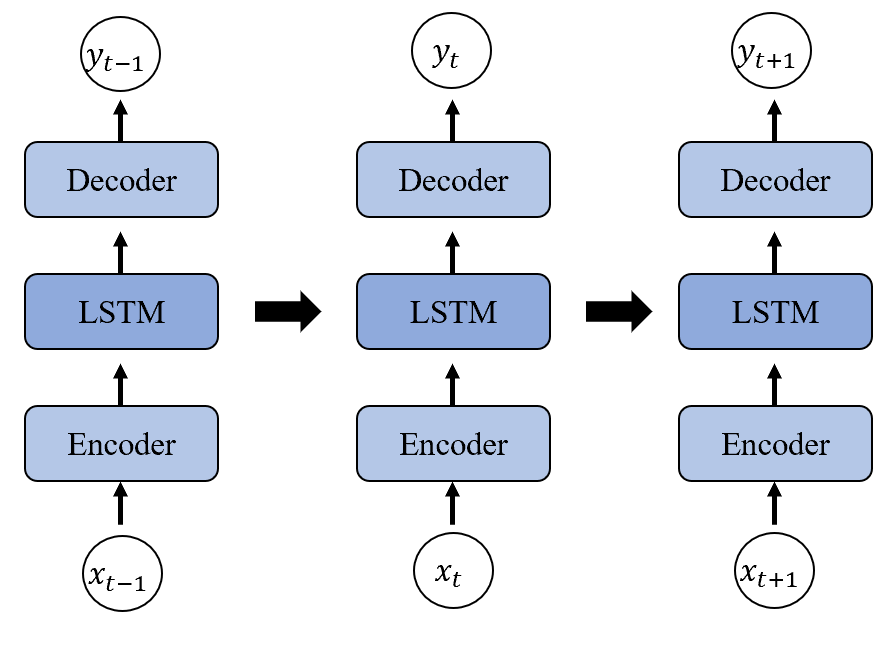
\includegraphics[width=0.6\textwidth]{FigMa/EDR.png}\\
    \vspace{-0.3cm}
    \caption{EDR 网络结构}
    \label{fig:EDR}
\end{figure}
其中$x_t$代表第$t$个时刻的输入的人体姿态,而$y_t$则代表由$x_t$预测出的未来人体姿态。网络接受$x_i$作为每个RNN节点的输入。具体的,输入姿态由编码器(Encoder)编码到隐空间,随后送入RNN层,提取到的时序信息,一路传递给下一个节点。另一路传递给解码器(Decoder),解码出对应的未来人体姿态作为当前节点的输出。该方法很好地利用了RNN的时序数据建模能力,有效提取了输入人体运动序列中的时序信息。但由于预测时需要参考上一个时刻的隐状态预测当前时刻的运动,因此容易出现误差累积问题。此外,由于在EDR中,未来运动序列被逐时刻、独立地预测,因此在输入序列和预测序列的过渡部分容易出现不连续的现象。
\begin{figure}[ht]
    \centering
    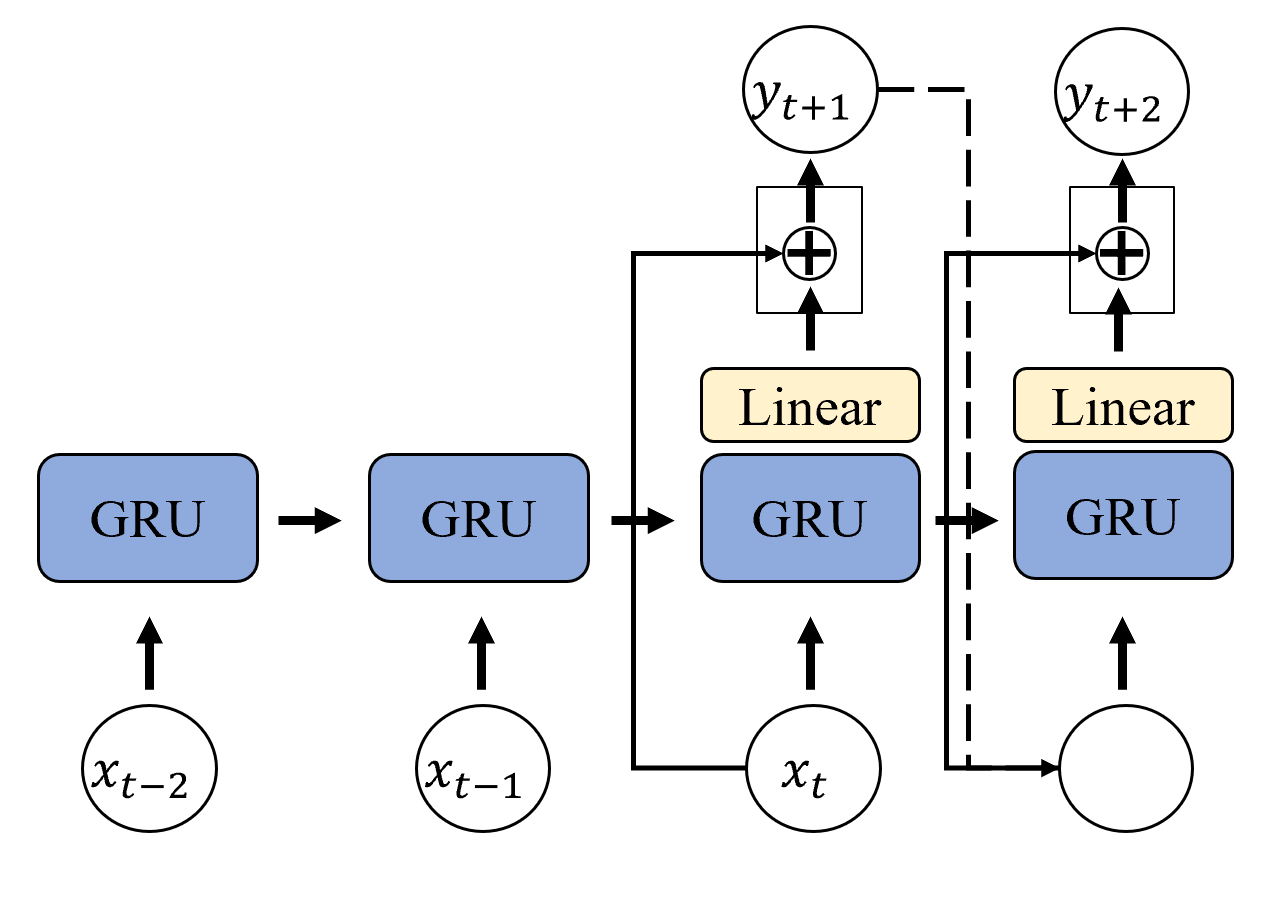
\includegraphics[width=0.6\textwidth]{FigMa/ResSup.png}\\
    \vspace{-0.3cm}
    \caption{Res. Sup. 网络结构}
    \label{fig:ResSup}
\end{figure}
Res. Sup.\parencite{martinez2017human}针对EDR中的问题提出了改进措施,如图\ref{fig:ResSup}所示,Res. Sup.引入了在自然语言处理领域常用的$seq2seq$模型结构,与EDR相比,$seq2seq$统一将输入序列编码到隐空间,此时隐空间包含所有的历史信息,这有助于模型从全局的角度考虑,而不是主要依靠当前时刻的输入,可以保证预测序列的一致性。随后,通过解码器,隐空间中的信息被解码为未来人体运动,在这个过程中,当前时刻的输出将作为下一时刻的输入,也允许相邻时刻的运动通过残差连接的方式完成一致性约束。除网路结构外,另一些方法从人体运动学入手,通过分析人体运动模式来针对性地设计网络,例如Tang \etal \parencite{tang2018long}发现在人体运动中,并非所有关节点都处于频繁运动状态。相反只有处于肢体末端的关节点位置才会较为频繁地改变。因此,它们提出要重点人体运动模型中频繁运动的关节点,称为HUM。具体的,他们设计了一个新颖的门控单元用来过滤运动幅度小的关节点。此外,注意力机制也被用来关注具体的运动模式。AHMR\parencite{liu2022investigating}为了捕获更多的长期相关性,在RNN单元中,可以同时对相邻关节和帧进行编码。此外,它不仅可以同时对本地和全局上下文进行建模,而且还使用了一个注意力模块来帮助更新全局上下文。

虽然上述方法在EDR的基础上提出了改进措施,提升了网络性能,但由于RNN网络的固有缺陷仍然无法解决诸如误差累积、过渡部分不连续、训练困难和难以处理长时间依赖关系等问题,这将削弱预测结果的精确性。为此一些新的方法的将目光投向了效率更高,感受野更大的卷积神经网络。

\section{基于卷积神经网络的人体运动姿态预测算法}
人体运动序列数据包含时间和空间两个维度,而卷积神经网络(CNN)在处理平面空间数据上有天然优势,时序信息也可以由1D的CNN(TCN\cite{oord2016wavenet})进行处理,相比循环神经网络,TCN更轻量化、推理速度更快、配合空洞卷积\cite{yu2017dilated}感受野更大。在人体运动姿态预测中,对于处理空间和时间的依赖关系是一个非常重要的问题。传统的CNNs只能捕捉静态图像的空间依赖性,但是在动态场景下,时间信息也是非常关键的。因此,研究人员提出了一些新的CNN架构,以同时处理人体运动预测的时空依赖关系。

在Butepage \etal \parencite{butepage2017deep}中,作者设计了一种新的卷积层来编码不同的时间尺度。这种卷积层可以有效地捕捉局部时间尺度的依赖关系,但是它无法处理长期的时间依赖性。为了解决这个问题,QuaterNet\parencite{pavllo2018quaternet}引入了扩张卷积,可以在网络中捕捉长期时间依赖关系。该方法在分层输入姿势的情况下表现良好,但仍然无法处理空间依赖性。

为了同时处理空间和时间的依赖性,一些研究人员采用了分层结构的CNN, Li \etal \parencite{li2018convolutional}利用卷积结构来捕捉长期隐藏状态,并将其送到解码器中以生成人体姿势。这种方法可以有效地处理时空依赖关系,但是它需要大量的计算资源和训练数据。为了进一步提高模型的性能,Li \etal \parencite{li2019efficient}提出了一种卷积分层自编码器框架,用于表示人体骨骼结构。在这种框架中,分层拓扑被用于表示骨骼结构,并且嵌入了1D卷积层来编码每个节点。因此,该框架可以有效地捕捉空间和时间的依赖关系。最近,TrajectoryCNN\parencite{liu2020trajectorycnn}被提出来处理人体运动预测的时空依赖关系。它引入了一种新型的轨迹空间,可以轻松地捕捉各种局部-全局的时空特征。这种框架在许多基准测试中取得了优异的性能。

虽然CNN能有效处理时间和空间数据,但CNN卷积核的规则结构决定它适合处理图像或视频这类规则数据。人体姿态属于不规则的无向图结构,人体关节点对应图中的顶点,骨骼对应顶点间的相互关系。这种拓扑结构是极其重要的先验空间信息,能有效辅助模型感知运动模式。而CNN的规则卷积核使得它很难利用这类先验信息。因此,在最近的研究中,天然具有拓扑信息处理能力的图卷积网络(GCN)获得了越来越多的关注。


\section{基于图卷积网络的人体运动姿态预测算法}
GCN是一种可以处理不规则图结构数据的神经网络。在GCN中,卷积操作是基于邻居节点之间的连接进行计算的,这使得GCN可以有效地处理具有不规则连接的数据结构,例如人体关键点。此外,GCN还可以利用拓扑信息来捕捉节点之间的关系,从而更好地理解图结构数据。该特性对人体运动序列数据处理非常有利。

%LTD DMGNN ST-GCN 
\begin{figure}[ht]
    \centering
    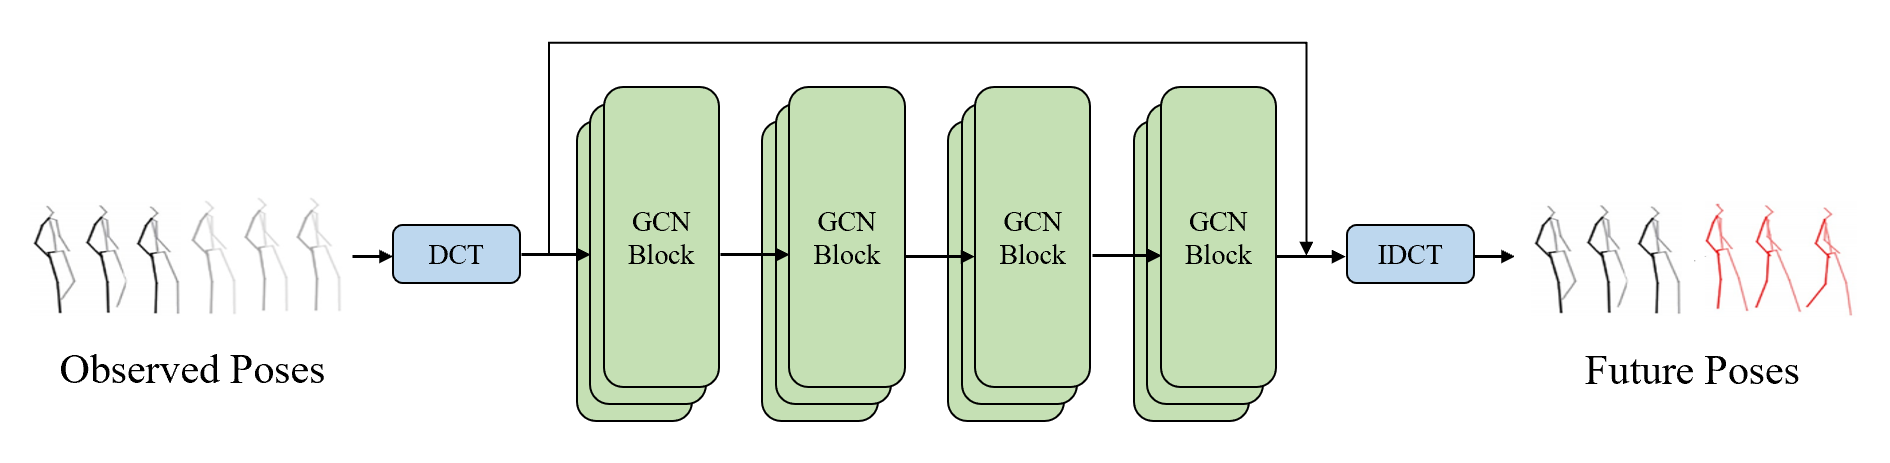
\includegraphics[width=1\textwidth]{FigMa/LTD.png}\\
    \vspace{-0.3cm}
    \caption{LTD 网络结构}
    \label{fig:LTD}
\end{figure}
LTD\parencite{mao2019learning}率先提出了一种代表性的GCN方法(图\ref{fig:LTD}),它使用原始的GCN对人体运动序列进行建模。具体的,对于输入的人体运动序列,LTD将其视作一个不规则的无向图。由于人体运动序列数据包含时间和空间两个维度,而原始的GCN只能处理二维平面数据。因此,LTD将该运动序列中的关节点轨迹视作一个整体,将其放入图结构网络中。即图中的每个节点包含了某个关节点这段时间内的运动轨迹,由此LTD使用一个描述平面拓扑结构的GCN来处理时空维度的人体运动序列。在结构方面,网络接受历史人体运动序列作为输入,为了保证输入数据和输出数据在时间维度上的一致性,LTD提出用已知序列的最后一个人体姿态填充输入序列,使其与输出序列时序长度一致。此外,网络输入和输出数据之间的残差连接也得到保证,有助于提高网络的训练效率和预测精确性。完成填充步骤后,输入数据将经过离散余弦变换(DCT)从时域变换到频率域,通过过滤掉低频信息保留高频信息,可以在降低数据维度的同时减少噪声。随后,变化后的特征被传入多个串联的GCN模块,进行特征提取步骤。最后,经过离散余弦逆变换(IDCT)后,输出最终的预测结果。该方法的贡献在于,提出了一种使用原始GCN对时序数据进行建模的方式。此外,全局的残差连接解决了输入序列和预测序列过渡部分的不连续问题,在最终预测精度上大幅领先基于RNN的方法。但由于该方法忽略数据的时序特性,仅仅使用GCN提取人体姿态的空间结构信息,将关节点轨迹作为一个整体放入图节点中,这导致该模型对时序运动的感知能力有所欠缺。

用于人体姿态提取的方法ST-GCN\parencite{yan2018spatial}针对LTD中存在的问题,提出了一种具有时空信息提取能力的GCN。对于时空人体运动序列数据,一个直观的想法是建立一个包含时空维度的邻接矩阵,囊括不同时间和空间上的关节点。但由于GCN复杂度随着时空维度的增加成倍数上升,该建模方式的复杂度是难以接受的。因此ST-GCN提出将数据的时间和空间维度分离,分别用TCN\parencite{oord2016wavenet}和GCN进行处理。具体的,1D的卷积神经网络TCN负责提取各个关节点轨迹中的时序信息,GCN负责处理人体姿态中的空间结构信息。通过将时空两个维度拆分,ST-GCN实现了线性增长的时间复杂度。并且通过实验证明网络时空信息提取能力优于现有方法。但TCN为局部特征提取算子,感受野被限制在卷积核范围内,导致ST-GCN在提取长时依赖上存在缺陷。

最近MSR\parencite{dang2021msr},设计了一种在空间维度上的多阶段GCN网络。它提出了一个类Unet\parencite{ronneberger2015u}网络。编码器部分,逐渐简化人体姿态空间结构,逐渐降低空间上的复杂性。解码器部分,首先预测空间结构较简单的人体运动序列,随着网络的深入,人体运动序列的空间复杂程度逐渐增加,直到输出具有完整空间结构的数据。在GCN特征提取模块设计方面,它参考了LTD,将关节点运动轨迹视作一个整体。该方法提出的空间层次化Unet网络,设计了一个渐进式的学习过程,这有利于降低每一阶段网络的学习难度。但对空间结构进行简化的过程中,破坏了人体结构先验信息,导致网络预测精确性相比LTD并没有明显提升,某些方面甚至出现了下滑。

由于GCN网络对图结构数据中节点关系的处理具有先天的优势,因此GCN能够更好地提取人体姿态数据中的结构先验信息。但现阶段的GCN的时空跨维度信息处理能力仍然有所不足。它们或是忽略某一个维度来降低时间复杂度,或是在信息提取能力和时间效率上做出了妥协。因此,如何平衡模型复杂度和时空信息处理能力,将是当前研究过程中的一个重要课题。

\section{基于对抗生成网络的人体运动姿态预测算法}
人体运动姿态预测算法的一个主要难点在于,预测过程中存在不确定性,这种不确定性是由于输入序列和预测目标序列之前的差异造成的。例如,如果输入序列与待预测序列之间的关联性强,则预测越简单,反之则越难。针对上述问题,一个解决思路是如上述方法,通过提高网络的时空信息提取能力,尽可能捕捉输入和预测序列间的关联性。另一个思路是引入生成式模型和随机性,生成更真实的、更多样化的运动序列。具体的,近年来由于对抗生成网络\parencite{goodfellow2020generative}的深入研究,GAN为生成人体运动姿态序列提供了更多的可能性。

Barsoum \etal \parencite{barsoum2018hp}率先提出了一种基于GAN的$seq2seq$人体运动序列预测方法,它使用改进版的WGAN-GP进行训练,与上述基于RNN,CNN或GCN的方法不同,它的网络输出为概率密度分布而非固定的人体运动序列。因此,在预测时可以通过为网络提供不同的随机噪声$z$,来对同一个输入运动序列预测不同的未来运动序列。然而,虽然该方法在结果真实性方面有所提升,但由于输入噪声的引入,预测准确性有所下降。在此基础上,BiHMP-GAN\parencite{kundu2019bihmp}同样通过在输入序列中添加从固定分布中采样的随机噪声来为预测过程添加随机性。不同的是,BiHMP-GAN提出了一个双向对抗神经网络来解决预测过程中的模式坍塌问题。
与此同时,受到上述工作的启发,AGED\parencite{gui2018adversarial}提出了一种新颖的对抗生成框架,它具有两个全局的循环鉴别器,一个鉴别器被用于促进生成序列的保真度,另一个鉴别器与网络进行联合训练,保证未来生成序列的连续性。STMI-GAN\parencite{hernandez2019human}也沿用了该思路,用于处理长时依赖的人体运动序列。ARNet(Adversarial Refinement Network)\parencite{chao2020adversarial}设计了一种新的对抗式的误差调整策略,与上述方法不同的是。判别器不再直接判断生成结果的真实性而是用来估计预测误差,随后精修模块再根据误差调整预测结果。而Lyu \etal \parencite{lyu2021learning}则利用GAN模拟路径积分来解决随机微分方程并预测未来运动轨迹。值得注意的是,由于对抗训练特性,想要训练达到平衡状态是非常困难的,Cui \etal\parencite{cui2021efficient}提出了一种新的GAN,该GAN使用了Spectral归一化以避免模式坍塌。还有另一种称为AMGAN\parencite{liu2021aggregated}的策略,它由复合GAN结构设计而成,包含用于不同低维身体部位的局部GAN和用于高维全身的全局GAN组成。该方法证明了降维可以有效地提高GAN的训练效率。

总而言之,利用GAN的策略主要可分为两类。(1) 通过对抗学习策略帮助网络生成更加真实的结果。(2) 利用随机噪声向网络添加随机性,生成多样化的预测结果。而GAN作为一个具有明显优势和劣势的网络,也会给研究人员的工作带来一定的挑战。


近些年,Transformer受到了学术界的广泛关注,它也从自然语言处理(NLP)领域被引入到计算机视觉领域,在诸如图片识别、图片分割等经典问题上大幅领先现有的基于卷积神经网络的方法。对于人体运动序列预测问题,网络需要捕捉长时依赖关系的能力。而Transformer的全局感受野特点恰好可以解决该问题。因此出现了一批基于Transformer的方法\parencite{aksan2021spatio, cai2020learning}。

Aksan \etal \parencite{aksan2021spatio}设计了一个包含时间和空间分支的Transformer网络,两个分支分别提取输入序列的空间结构信息和时序信息,最后再通过融合模块得到最后的预测结果。


\section{基于Transformer的人体运动姿态预测算法}
\begin{figure}[ht]
    \centering
    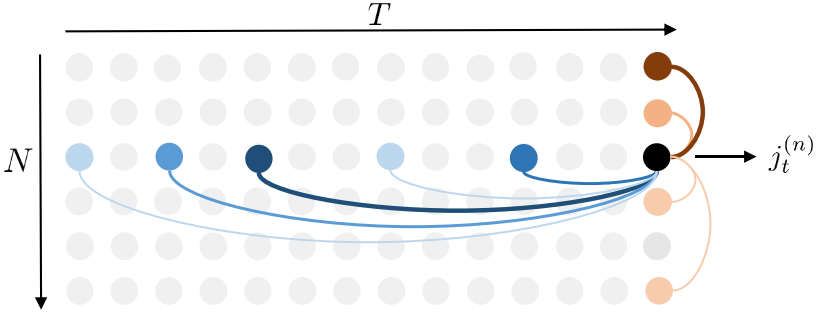
\includegraphics[width=0.6\textwidth]{FigMa/ST-Transformer.png}\\
    \vspace{-0.3cm}
    \caption{Spatiotemporal Transformer\parencite{aksan2021spatio}中的时空特征提取方式}
    \label{fig:Spatial-temporal_Transformer}
\end{figure}
其中Spatiotemporal Transformer时空特征提取策略由\ref{fig:Spatial-temporal_Transformer}所示,$j^{(n)}_t$表示$t$时刻,第$n$个关节点。其中,$j^{(n)}_t$只和自己位于同一时间或空间的关节点进行注意力(Attention)机制计算,图中颜色的深浅代表关节点之间的关联程度,颜色越深关联性越强,权值也越高,反之则越小。通过分离的时空transformer,该方法间接地提取了全局的时空信息。

\begin{figure}[h]
    \centering
    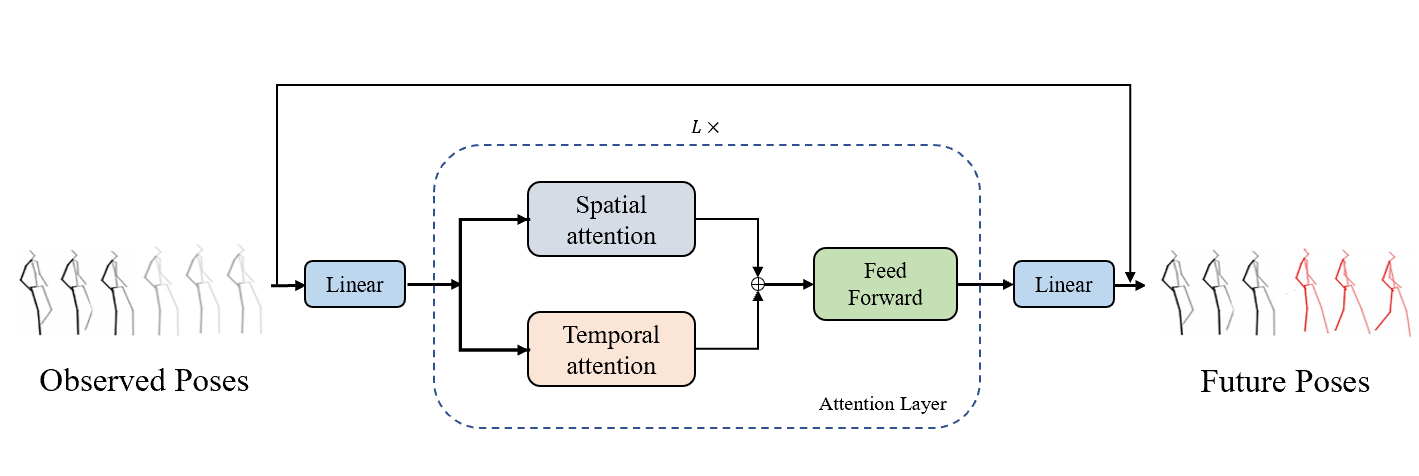
\includegraphics[width=1\textwidth]{FigMa/ST_Transformer.png}\\
    \vspace{-0.3cm}
    \caption{Spatiotemporal Transformer\parencite{aksan2021spatio}网络结构}
    \label{fig:Spatial-temporal_Transformer_structure}
\end{figure}
完整的网络结构如图\ref{fig:Spatial-temporal_Transformer_structure}所示,网络由$L$个串联的注意力层构成,每个层包含一个并行的空间维度和时间维度的注意力层,特征被传入注意力层后,分别送往两个分支,用于提取时间和空间信息。提取结束后,空间和时间信息相加,送入前馈神经网络进行特征融合,最终通过线性层输出预测的未来人体运动序列。该方法通过并行的方式分离时间和空间维度,减少了时间复杂度和模型参数量。但并行的方法使得时间和空间维度缺少信息通信手段,导致信息交流受阻,影响最终的预测质量。总的来说,Transformer高效的全局注意力机制有利于模型捕捉长时序依赖,但Transformer的注意力计算模块也导致模型空间的上升和计算开销的增加。此外,时间和空间分支间的通信问题也是未来需要研究的问题。

%看情况还写不写另一个方法的介绍。

\section{总结}
本章,本文对人体运动姿态预测算法的发展做了一个简要的回顾。在初期,研究人员根据循环神经网络在处理时序数据上的优势,设计了基于RNN的人体运动姿态预测模型来对输入序列编码后预测未来运动序列。但由于循环神经网络对于时序记忆的能力依赖隐变量的大小,因此难以处理长时依赖。此外,梯度消失等训练问题也困扰着现有方法。随后,研究人员将目光转向了卷积神经网络,特别是图卷积神经网络,它在不规则的拓扑结构数据处理上有天然的优势。但如何对传统图卷积网络进行改进,使其拥有高效的时空信息处理能力,仍然是当前的研究热点。此外,GAN机制的引入允许生成更多样化和真实的结果,但其训练过程的不稳定性和噪声对结果准确性的影响有待进一步解决。近些年,Transformer的兴起给该问题带来了新的解决思路,其全局感受野的特性,允许其捕捉更长范围的全局依赖。但其注意力计算带来的额外计算开销和时空信息间的通信问题,还需要进一步探索。本文希望在现有基于图卷积的方法的基础上,提出一种新颖的人体运动姿态预测算法,有效提高模型的时空信息提取能力,并且控制模型的运行开销。


